\documentclass[a4paper, onecolumn, 12pt]{IEEEtran}
%\documentclass[draftcls, onecolumn, a4paper, twoside]{IEEEtran}

% Prepared by Dr H. Laue for EJJ 210 Professional and Technical Communication. Latest revision: May 2022.

% Acknowledgement: Many of these guidelines are based on the Departmental guidelines for practical reports dated September 2015. 

% This \LaTeX\ template was adapted by Ms Liebet Joubert from previous work by Dr H. Laue and Prof. W.P. du Plessis. Last revision: February 2023.


% These values get used many times, so it is easier to define them once here.
% Module code
\def\modulecode{EAI 320}
% Module name
\def\modulename{Intelligent Systems}
% Assessment title
\def\assessment{Practical 4}
% Group number
\def\groupnumber{ }

% Student details: (Leave blank the last student(s) if your group has fewer people. The contributions MUST add up to 100%. Additional rows in the table on the title page can be commented out in titlepage.tex.)
% Details of the first student
\def\firststudentname{Moosa Osman}
\def\firststudentnumber{24566722}
\def\firststudentcontribution{100}
% Details of the second student
% \def\secondstudentname{Second Student}
% \def\secondstudentnumber{23456781}
% \def\secondstudentcontribution{50}

% Allows multi-line equations to be split over a number of pages.
\interdisplaylinepenalty=2500 

%% Include packages in the user_packages.tex file to declutter the report.tex file where you will be working.
\input{user_packages.tex}

% Set the PDF properties of the document.
\hypersetup{%
  pdftitle={\modulecode -- \assessment},
  % pdfauthor={Group \groupnumber}}
}
\begin{document}

% Try to keep text inside the right margin.
\sloppy

% Formatting of the code environments and bibliography are included in the user_formats.tex to declutter the report.tex file where you will be working.
\input{user_formats.tex}

% Title page
% Title page

\newcolumntype{A}{>{\centering\arraybackslash}m{4cm}}
\newcolumntype{B}{>{\centering\arraybackslash}m{3.75cm}}
\newcolumntype{C}{>{\centering\arraybackslash}m{3.25cm}}

\begin{titlepage}
    \begin{center}

        \vspace*{2cm}
    
        % University Logo
        
\includegraphics[width=0.6\textwidth]{drawings/up_logo_ebit.pdf}\\[2.0cm]    
    	
        % Department Title
        \textsc{\LARGE\bfseries \modulecode}\\[1.0cm]
    	
        % Module Tile
        \textsc{\Large\bfseries \modulename}\\[0.75cm]
    
        % Assignment Title
        \textsc{\large\assessment}\\[0.5cm]
        
        %Group Number
        % \textsc{\large Group \groupnumber}\\[1.0cm]
        
    		
        % Students/Contributors Table
        \begin{table}[h]
            \centering
            \normalsize
            \begin{tabularx}{\textwidth}{|A|C|B|C|}
                \hline
                \textbf{Name and Surname} & \textbf{Student Number} & \textbf{
\includegraphics{figures/Osman M signature.png}} & \textbf{\% contribution} \\
                \hline
                & & &   \\
                \firststudentname   & \firststudentnumber   & & \firststudentcontribution \\ 
                & & &   \\ \hline 
            \end{tabularx}
        \end{table}
		
    \end{center}

  % Report Declaration
%   Comment this line out and uncomment the line below it in the \verb|report.tex| file to include the required declaration.
    \noindent By submitting this assignment we confirm that we have read and are aware of the University of Pretoria's policy on academic dishonesty and plagiarism and we declare that the work submitted in this assignment is our own as delimited by the mentioned policies. We explicitly declare that no parts of this assignment have been copied from current or previous students' work or any other sources (including the internet), whether copyrighted or not. We understand that we will be subjected to disciplinary actions should it be found that the work we submit here does not comply with the said policies.
    
    % Include the declaration below instead if you work alone.
    
    % \noindent By submitting this assignment I confirm that I have read and am aware of the University of Pretoria's policy on academic dishonesty and plagiarism and I declare that the work submitted in this assignment is my own as delimited by the mentioned policies. I explicitly declare that no parts of this assignment have been copied from current or previous students' work or any other sources (including the internet), whether copyrighted or not. I understand that I will be subjected to disciplinary actions should it be found that the work we submit here does not comply with the said policies.
	
    \vfill
  
    % This is useful for sending papers that have been rejected to people outside the university.
    \scriptsize%
    \noindent%
    \copyright~\number\year{} University of Pretoria \\
    This contains information which is confidential and proprietary to the University of Pretoria (``the
    University''). The information contained herein is to be used exclusively by you for the purpose for which it was disclosed by the University and may not be disclosed to anyone or be used for any purpose other than as set out above, without the University’s prior written consent.%

    % \vfill
    % \begin{center}
    %     \large\today
    % \end{center}

\end{titlepage}

%% Avoid expanding abbreviations.
%\glsunsetall
% Ensure that the abbreviations are expanded in the text.
% \glsresetall

% Table of Contents
% \pagenumbering{roman}
% \pagestyle{plain}
% \setcounter{tocdepth}{2}
% \addtocontents{toc}{\protect\thispagestyle{plain}}
% \tableofcontents
% \clearpage
\pagenumbering{arabic}
\setcounter{page}{1}
\pagestyle{fancy}


% \section{Introduction}
% \label{sec:introduction}

% Most of the written assignments that undergraduate students in the Department will encounter are in the form of practical reports. Therefore, it is crucial that they learn how to write high-quality practical reports, as they will need this skill not only in their undergraduate studies, but throughout their entire career.

% Reports come in many forms, and it is often challenging to select the appropriate outline for your report. This template follows the standard model for scientific reports, which follows the outline of Introduction, Theoretical Background, Method, Results, Discussion, and Conclusion. The main exception is that the Method section can be renamed to Design, as engineering assignments often involve design and not only experiments.

% This template aims to teach students how to write high-quality reports in the format required by the Department. Since some of the formatting requirements can be tricky to get right, the template makes use of several examples to illustrate how the required formatting can be achieved. It is expected that students who make use of this template and follow its guidelines will achieve above-average marks for their practical reports.

% Consider the three paragraphs above as an example of a well-written introduction. 

% \textit{Paragraph 1}: Pay special attention to your first paragraph. It should introduce the topic being addressed in the report in terms of its \textit{significance to your audience}. It should answer the question, `So what?' In this case, you might ask, `So what? Why do I need to learn about practical reports?' in which case the first sentence answers that question by stating that you will encounter them throughout your undergraduate career. The rest of the paragraph elaborates on the implications of the first sentence.

% In general, you can assume that you have a technical audience, i.e. engineers, but not necessarily specialists in the subject at hand.

% \textit{Paragraph 2}: Next, zoom in slightly and present the context of the problem – where your topic finds itself within the greater subject area (`Reports come in many forms … This template follows the standard model for scientific reports'). For practical reports, this should not be more than a few sentences. Use words only and avoid the excessive use of acronyms or technical jargon that your audience does not yet understand – the next section is for explaining those concepts. If you reach the point where you want to include an equation or a figure, you have gone too far.

% \textit{Paragraph 3}: Next, state what the aim of the investigation was (`This template aims to teach…'), how the task was approached (`…the template makes use of several examples to illustrate…'), and what the expected outcomes were (`It is expected that students who make use of this template…'). In general, one states the aim of the report or paper (`This report presents…'), but for practical reports it is acceptable to refer to the aim of the practical instead (`The aim of this practical was to…'). Again, keep it short and simple.

% Throughout the report, write in the past tense and in third-person passive. For example, `The measurement was taken', not `I took the measurement'.

% In longer reports, papers, or chapters in theses and dissertations, one typically ends the introduction with a paragraph giving an outline of the remainder of the work, e.g. `The remainder of the report is structured as follows. Section 2 presents the theoretical background for … In Section 3, the details of the design, simulation and implementation are given…' However, this is not generally required for practical reports.

% Try to keep your introduction about half a page long, and no longer than a full page.

% \section{Theoretical Background}
% \label{sec:theoretical_background}

% The aim of this section is to provide more detailed theory that is required to understand the rest of the practical. Here you can introduce equations, circuit diagrams, and illustrations to explain the concepts. Only provide the essentials that you will use in the following sections. Refrain from delving into concepts that are not relevant to the practical at hand, or deriving all of the mathematics from first principles (unless specifically instructed to do so); you should present a reference that your readers can consult for the detailed derivations.

% Do not present any calculations specific to your experiments or your design (with numeric values); this will be covered in Section~\ref{sec:design}. Generally, circuit diagrams provided as part of the theoretical background should not include component values, only component names.

% Equations should generally be referenced at the end of the preceding phrase. For example, Ohm's law is given by equation \cite{ohm}\footnote{Include the sources in the `references.bib' file and then cite them where relevant in the text. This will automatically include them in the References list in the correct order.}
% \begin{align}
%     V   &= IR, \label{eq:ohms_law}
% \end{align}
% where \textit{V} is the voltage in volts, \textit{I} is the current in amperes, and \textit{R} is the resistance in ohms. Note the comma after the equation, since a comma is required as per the normal rules of grammar. Also, note how all the variables/symbols in the equation are defined in the text. In most cases, a reference will be required for each equation when dealing with the theoretical background. Your own calculations in Section~\ref{sec:design} will, of course, not each have a reference. In the rare case that you follow a detailed derivation from a particular source, you can start the derivation with a statement such as `The following derivation follows \cite{ohm}' to avoid having to place a reference before each equation. However, be careful not to plagiarise the words in between the equations – you still need to explain the derivation in your own words.

% Take care to explain the concepts in your own words and not commit plagiarism. Make sure to cite your sources and to use quality sources. Your textbook should be a good source to consult. Draw your own diagrams from your own understanding of the concepts as far as possible, even if they are only simple representations. You can use tools such as \href{https://www.diagrams.net/}{diagrams.net} to create your own diagrams

% The best way to avoid plagiarism is to first have a solid understanding of the subject. Unfortunately, there is no shortcut around this, and not understanding a source properly is the surest way to commit plagiarism, because you will not be able to explain the concepts in your own words. Think about your everyday conversations, and how often you retell a story that you either heard or read. Chances are that you do a very good job of telling the story in your own words, because you don't have the original source there with you, and we are not generally good at remembering things word-for-word. \textit{Therefore, the greatest barrier to proper paraphrasing is not your ability to put things in your own words, but rather your understanding of the source itself.} If you do not fully understand a source, rather do not use it. 

% In general, explicit permission is required to reuse copyrighted material, e.g. figures or tables, in your own work, unless the material is in the public domain or released under a licence that allows reproduction (e.g. a \href{https://creativecommons.org/licenses/}{Creative Commons licence}). Some journals are released under Creative Commons or similar licences, but most are not, and almost no textbooks are. Even if you redraw a figure, you are still copying the original work! Some copyright licences specifically prohibit modification (derivative works), even if the licence allows you to freely reuse the work in its original form. See \href{https://library.up.ac.za/c.php?g=615261&p=4278756}{this page} on the \ac{UP} library website for more information on the use of copyrighted works.

% There is one exception to the rule above, and that is that you are allowed to reuse copyrighted material (figures, tables, etc.) in reports that you submit for the purpose of evaluation (i.e. university assignments) without requesting permission, provided that they are not published anywhere. However, a word of caution: Be careful of getting into the habit of using copyrighted material in your reports. Once you are done with your undergraduate degree, you will need to apply for permission to reuse every single piece of copyrighted material (that is not released under a free-use licence) in almost any report you write. So, before using a copyrighted figure in your university report, ask yourself whether it would still be worth including the figure if you needed to apply for permission. If you do use a copyrighted figure, make sure that the quality of the figure you are including is up to standard; do not include low-resolution screenshots and do not include parts of the caption in the screenshot. 

% Copyrighted figures and tables require not only \textit{citation}, but also \textit{attribution}. Citation acknowledges the author of a source so that nobody gets the impression that it was your idea, whereas attribution is an acknowledgement of the copyright holder of a work. Failing to cite a source results in \textit{plagiarism}, an ethical violation, whereas failing to attribute copyrighted material results in \textit{copyright infringement}, a legal violation.  Citation is done by means of an entry in the reference list and an in-text citation (e.g. \cite{ohm}), whereas attribution is done by means of a declaration at the end of a figure or table caption (e.g. \textcopyright~2022 IEEE). Below are two examples of both citation and attribution according to the requirements for IEEE-copyrighted works.
% \begin{itemize}
% 	\item Taken from \cite{ohm}, \textcopyright~2022 IEEE.
% 	\item Adapted from \cite{ohm}, \textcopyright~2022 IEEE.
% \end{itemize}
% An example is shown in \figurename~\ref{fig:copyright}. Note that the caption text should be justified. The same applies to tables, as shown in \tablename~\ref{tab:voltage_comp}.

% The first example is for figures or tables reproduced in their original forms, and the second example is for derivative works, e.g. redrawn or modified figures.

% Aim to keep this section between one and two pages long.

% \begin{figure}[htbp]
%     \centering
%     
\includegraphics[width=0.35\textwidth]{figures/copyright.png}
%     \caption{The copyright symbol. Taken from [X], \textcopyright~YYYY Copyright Holder.}
%     \label{fig:copyright}
% \end{figure}


% \section{Method}
% \label{sec:method}

% This section contains all the details of your design and/or experimental setup. The guiding principle is that anybody should be able to recreate your results exactly by following the steps you present here.

% A practical assignment may consist mainly of experiments, where you are tasked with investigating the effect of one variable on another, or may focus on the design of a component, circuit or device. Your approach to this section will differ slightly based on the type of practical assignment.

% In both experimental and design-focused practicals, you will usually compare the results of your experiments/design at the levels of theory, simulation, and measurement. You are free to change the sub-headings in this section, especially for design-focused assignments, but try to keep to the outline of theory-simulation-measurement as far as possible. The subsections should follow a logical progression in terms of your methodology, from theoretical calculations through to your measurement setup.

% Write a short introductory paragraph here to avoid having a subsection immediately below a section heading. Give an overview of the methodology that will be followed for the practical.

% \subsection{Theoretical calculations [or] Design}
% \label{sec:design}

% Based on the theory, what results do you expect from your experiment/design? This sub-section is where you present the theoretical calculations that indicate what the expected results are. In the case of a design-focused assignment, this is where you present your theoretical design, including assumptions, calculations, and circuit diagrams.

% Be careful not to confuse this sub-section with Theoretical Background. In Theoretical Background, you describe the theoretical principles in general terms, i.e. in terms of variables and circuit components, without specifying any particular values. Here, you now specify the exact values that you will be using in the practical:
% \begin{itemize}
%     \item Where you presented equations in terms of variables in Theoretical Background, now specify the values of the variables and calculate the theoretical results.
%     \item Where you presented circuit diagrams with component names only, now present the actual component values that you will use in the practical.
% \end{itemize}
% In many cases, it is possible to calculate the expected results mathematically. For example, if you are investigating Ohm's law, you could say:

% One 100\,$\Omega$ resistor was provided and an ammeter was to be connected in series with the resistor and a 9\,V battery. The expected current I can be calculated by rearranging \ref{eq:ohms_law} to give
% \begin{align}
%     I   &= \frac{V}{R} \label{eq:ohm_rearranged} \\
%         &= \frac{9}{100} \label{eq:calc_current} \\
%         &= 0.09 \text{ A} \label{eq:current_amp} \\
%         &= 90 \text{ mA.} \label{eq:current_mA}
% \end{align}

% Note how the equals signs are aligned (use `align' instead of `equation'), and how the units A and mA are upright and not italicised (include the text within the curly braces of `\textbackslash text\{\}').

% \subsection{Simulation setup}
% \label{sec:sim_setup}

% The subsection describes the procedure for setting up your simulations but does not yet present any simulated results. However, you can mention some observations that informed the final design. You are allowed to present screenshots here if such screenshots are helpful to explain how you set up the simulations -– remember that the focus is on presenting your methodology.

% Explain step-by-step how you set up the simulation. What software did you use? What were the parameters of the various components? How did you set up the settings for the solver? Across which ranges did you evaluate the variables and why? Did you export the data from the software and if so, in which format? You generally do not need to include code. If you did something new or unique in your code, present only snippets of code here. If you are required to include all of your code, do so in an appendix unless instructed otherwise.

% If the practical was design-focused and involved a lot of back-and-forth between simulation and implementation, this sub-section can be merged with the next sub-section under the heading `Implementation'.

% \subsection{Measurement setup [or] Implementation}
% \label{sec:implementation}

% This subsection describes your experimental setup. In the case of a design-focused practical, this section gives details of the practical implementation (how you built the circuit or device), and your measurement setup.

% For practicals that focus on experiments, the title `Measurement setup' is suggested. For practicals that focus on designing and building a circuit, component, or device, you can use the alternative title `Implementation'.

% As with the method for simulations, somebody else should be able to replicate your measurements by following the steps you provide here. How did you build the circuit or device? What laboratory equipment did you use? How did you set it up? Across which ranges did you test the circuit, and why? What were the steps followed in the experimental procedure? How did you save the results?

% In general, it will not be necessary to provide a photograph of your measurement setup unless there is something particularly new or unique about the setup that you would like to illustrate. Similarly, photographs of your circuit are generally not required, but for design projects with physical constraints or an aesthetic component, such as a \ac{DC} motor, robot car, or fabricated antenna, you can include a photograph to illustrate some of the design decisions you made.


% \section{Results}
% \label{sec:results}

% In this section, present and compare your theoretical, simulated, and measured results using words, graphs, and tables. Each figure or table should have an in-text reference. For example, \tablename~\ref{tab:voltage_comp}\footnote{You can use \href{https://www.tablesgenerator.com}{Create LaTeX tables online} to generate tables.} compares the theoretical, simulated and measured voltage for circuits A, B and C. 

% \begin{table}[htbp]
% \centering
% \caption{Theoretical, simulated, and measured results for circuits A, B, and C.}
% \begin{tabular}{cccc}
% \hline
%         & \multicolumn{3}{c}{Voltage (V)}   \\ \cline{2-4} 
% Circuit & Theory & Simulation & Measurement \\ \hline
% A       & 0.50   & 0.52       & 0.63        \\
% B       & 1.50   & 1.49       & 1.44        \\
% C       & 2.00   & 2.10       & 2.09        \\ \hline
% \end{tabular}
% \label{tab:voltage_comp}
% \end{table}

% As far as possible, export all your oscilloscope measurements to text files and plot the results yourself. The ideal is to plot the theoretical, simulated, and/or measured results together.

% It is generally bad practice to simply `dump' all your figures and tables in this section without any comment. But how do you comment on the results if the Discussion section is dedicated to discussing the results?

% The key is to distinguish between making observations from your results, and discussing the significance of those observations. When you present a figure or a table in the Results section, you cannot assume that your reader will know what they are looking at. You need to comment on what the table or graph is showing and make some basic observations from the data. In other words, you need to `read' the table or graph. For example, it might be that as soon as you present the theoretical, simulated and measured results side-by-side, you notice that there is a large deviation in the measured results. In this section, you will then state that there is a large deviation and quantify that deviation. In the Discussion section, you will discuss the potential causes of the deviation and comment on the implications of the deviation. For example:

% \tablename~\ref{tab:voltage_comp} compares the theoretical, simulated and measured voltages for circuits A, B and C. All of the simulated and measured voltages deviated by 5\% or less from their theoretical values except for the measured voltage for circuit A, which was 26\% higher than the expected value.

% There are various phrases that you can use to compare values quantitatively:
% \begin{itemize}
%     \item Percentage (\%) higher/lower/deviation for values that you expect to be the same, e.g. theoretical, simulated, and measured values of the same parameter.
%     \item Difference in dB for values expressed in dB. Do not use percentages for comparing values in dB! For example, you cannot say that 1.1\,dB is 10\% higher than 1\,dB! In the case of a voltage, a 0.1\,dB increase is actually only 1.16\% higher.
%     \item Multiples for large differences, e.g. five times larger or 3.3 times smaller. Multiples are usually preferable to percentages larger than 100\%.
% \end{itemize}

% You can also compare values qualitatively using comparative words, as long as such descriptions are accompanied by quantitative descriptions as above. For example:

% \begin{itemize}
%     \item \textit{Significant, large, huge} (difference, deviation, discrepancy, etc.): When the difference is more than expected, implying that this will be discussed further under Discussion.
%     \item \textit{Comparable, similar, close to, almost the same as, nearly equal, slightly bigger/smaller/lower/higher}: When differences are due to normal, expected variations and do not require further analysis.
%     \item\textit{ Notable, surprising, unexpected, worrying}: These adjectives border on interpretation and should normally be reserved for the Discussion section.
% \end{itemize}

% You might be describing a value across a particular range, in which case you can use phrases such as:

% \begin{itemize}
%     \item \textit{Equal to, better than, less than, greater than, ranging from/to… from/to, across, below, above, beyond, outside}, e.g. `The amplitude was greater than 10\,dB from 0\,MHz to 5\,MHz'.
% \end{itemize}

% Be careful to distinguish between inclusive, e.g. [0,10], and exclusive, e.g. (0,10), ranges: 

% \begin{itemize}
%     \item Exclusive: \textit{greater than, less than, above, beyond, below, outside}, e.g. `distortion was observed for input voltages beyond 19\,V'. Note the combination of qualitative (`distortion) and quantitative (beyond 19\,V) expressions.
%     \item Inclusive: \textit{greater than or equal to, less than or equal to, from/upwards, from/downwards, 5\% or less, two or more, up to, up to and including, a maximum of, a minimum of}, e.g. in \tablename~\ref{tab:voltage_comp}, 2.1 is exactly 5\% more than 2, so you cannot say `deviations of less than 5\%', but you can say `deviations of 5\% or less'.
%     \item Ambiguous: \textit{between}.
% \end{itemize}

% There are various ways to present multiple values in writing. Be careful about the use of the word respectively.

% \begin{itemize}
%     \item `Circuit A had an expected voltage of 0.5\,V, circuit B had an expected voltage of 1.5\,V, and circuit C had an expected voltage of 2.0\,V.'
%     \item `Circuit A had an expected voltage of 0.5\,V; circuit B, 1.5\,V; and circuit C, 2.00\,V.' Note how in this case you want to keep the categories (A, B, and C) as close as possible to their corresponding values. Note the singular form `voltage'.
%     \item `Circuit A had theoretical, simulated and measured voltages of 0.50\,V, 0.52\,V, and 0.63\,V, respectively.' Note the plural form `voltages'. Note how in this case, you want to keep the values as close as possible in order to compare them.
%     \item `The measured voltages for circuits B and C were within 5\% of their respective theoretical values.' Note again the plural forms `voltages', `circuits', and `values'.
% \end{itemize}


% \section{Discussion}
% \label{sec:discussion}

% The aim of the Discussion section is to comment on and analyse the \textit{significance} of the results, and in particular, the reasons for and implications of any deviations in the simulated and measured results. Once you know what belongs in the Results section, pretty much everything else belongs here.

% The reason why it is good to have separate Results and Discussion sections is to avoid the temptation of thinking that making \textit{observations} is the same as interpreting the \textit{significance} of those observations, and you might end your report with `results' only. Having a dedicated Discussion section also helps avoid the temptation of using your conclusion for `discussion'.

% Firstly, consider the case where there were no unexpected deviations in the simulated or measured results. You can comment here that the minor variations are expected due to the tolerances of the components and instruments used as well as instrument noise. There might also be various `ideal' assumptions in theory that do not hold true in simulation and/or measurement; for example, a perfect square wave with an infinitely small rise time and zero over-shoot is not attainable in practice.

% Secondly, should there be significant deviations in your simulations or measurements, these need to be discussed in detail. What are the potential causes of these deviations? How can the experimental setup be changed to reduce the impact of these factors? For example, if a particular measurement is extremely sensitive to a particular resistance value, could it help to use a higher-precision resistor? You might need to perform some additional experiments to gain more clarity. If you performed extensive additional experiments, work these experiments into the rest of the report; do not present everything here.

% By the end of your discussion, it should be clear whether the desired outcomes of the practical assignment have been achieved.


% \section{Conclusion}
% \label{sec:conclusion}

% In the introduction, you started with the significance of the topic and worked your way towards what you would be doing in this practical. In the conclusion, you do the opposite: you start with what was done, and work your way towards the significance of what was discovered. In other words, if you read the introduction and conclusion only, you would know why the topic is important, what the aim of the practical was, what was done and what was discovered, and why these discoveries are important. In other words, you should be able to get the gist of the report from the introduction and conclusion alone.

% The conclusion should summarise what was done (method), the primary results obtained and observations made (results), the significance of those results and observations (discussion), and finally, why it matters to your audience (`So what?'). Since it is mainly a summary, there will be some overlap with the rest of the report, but the conclusion should not simply be a repetition of what was already said. Rather, it should focus on giving a holistic view of the practical. This becomes especially important as the length of the report increases. The aim is to reinforce what your readers have learned and why they should care. Doing this successfully will make your report both memorable and impactful.

% In this template, students have been shown how to write high-quality practical reports that meet Departmental requirements. This was done by means of guidelines, examples, and templates for the various components that make up a practical report. The standard model for scientific reports was found to be suitable for both experiment-focused and design-focused practicals, with some variation in the structure of the Method section to allow for differences between these two approaches. By applying the principles described in this template, students will not only learn how to write better laboratory reports but will learn written communication skills that will last them a lifetime.

% \textit{Prepared by Dr H. Laue for EJJ 210 Professional and Technical Communication. Latest revision: May 2022. }

% \textit{Acknowledgement: Many of these guidelines are based on the Departmental guidelines for practical reports dated September 2015. This \LaTeX\ template was adapted by Ms Liebet Joubert from previous work by Dr H. Laue and Prof. W.P. du Plessis. Last revision: February 2023.}



% Make the reference font the same size as the rest of the text.
% \IEEEtriggercmd{\normalsize}
% \IEEEtriggeratref{1}

% \bibliographystyle{IEEEtran}%
% \bibliography{references}%

% \textit{Follow the IEEE (recommended) or Harvard referencing style. Use \LaTeX's  bibliography manager to manage your citations. Include your sources in the `references.bib' file and cite them (\textbackslash cite\{\}) them in text. Remember that no reference manager is perfect, and that you still need to double-check that the references are formatted correctly, and make any changes as required.}

%\clearpage
\FloatBarrier


% Use for only one appendix (no titles necessary and no appendix numbers).
%\appendix
% Use for multiple appendices (with appendix numbers).
% \appendices


% \section{Abbreviations}
% \label{sec:abbreviations}
% \input{abbreviations.tex}

\section{Code}
\label{app:code}

% Use appendices to include code or data \textbf{\textit{if the instructions specifically ask for it}}.

% There are a number of \LaTeX{} packages for including source code in documents, and an example using the \verb|listings| package is included in \figurename~\ref{fig:code_listings}. The \verb|minted| package for including source code can also be used; an example is included in \figurename~\ref{fig:code_minted}.

% \begin{figure}[htbp]
%     \centering
%     \begin{lstlisting}
%     # Assignment X
%     # Group Y
%     # Name Surname 12345678
%     # Name Surname 23456781
    
%     import numpy as np
    
%     print('This is an example of using the listings package to include code.')
%     \end{lstlisting}
%     \caption{An example of including basic code using the listings package.}
%     \label{fig:code_listings}
% \end{figure}

% \begin{figure}[htbp]
%     \centering
%     \begin{minted}{python}
%     # Assignment X
%     # Group Y
%     # Name Surname 12345678
%     # Name Surname 23456781
    
%     import numpy as np
    
%     print('This is an example of using the minted package to include code.')
%     \end{minted}
%     \caption{An example of including basic code using the minted package.}
%     \label{fig:code_minted}
% \end{figure}

% When including code (especially longer sections) you would typically not include it as figures -- this was just done as an example here. Code can included outside of a figure by just using the \verb|lstlisting| and \verb|minted| commands directly instead of placing it inside a \verb|figure|. An example using the same code and the \verb|minted| package is shown here:

\begin{lstlisting}[language=Matlab, caption={Naïve Bayes classifier.}, label={app:code_impl}]
% Intelligent Systems EAI 320 Practical 4 (NAive Bayes)
% Moosa Osman u24566722
% Last updated: 20260516

function rps = agent_bayes(previous, n_rounds)
    persistent opponentHistory;
    persistent ourHistory;

    % General procedure:
    % Random for move one ==> start predicting based on previous moves
    %More moves ==> greater chance of predicting mvove properly
    % perform Naive Bayes and find most likely mvoe, then choose winning move

    if isempty(previous)
        opponentHistory = [];
        ourHistory = [];            % init the stuff
        
        rps = randi([0, 2]);        % play random first time
        ourHistory = [ourHistory; rps];
        return;
    end

    % update the history
    opponentHistory = [opponentHistory; previous];
    N = length(opponentHistory);

    %extracting the features
    f1Hist = opponentHistory(1:end-1);         % f1: Opponent's move 1 round ago
    f2Hist = ourHistory(1:end-1);          % f2: Our move 1 round ago
    cHist  = opponentHistory(2:end);            % C: Opponent's move this round

    currentf1 = opponentHistory(end);
    currentf2 = ourHistory(end);

    posteriorScores = zeros(3, 1);          % values fo the posteriors, to be used later
    totalSamples = length(cHist);         % no of samples 

    for idx = 1:3           % for all: need to find Cond. probs. 
        classVal = idx - 1;
                        
        countCk = sum(cHist == classVal);     % Count occurrences of the target class
                
        prior = (countCk + 1) / (totalSamples + 3);    %have to add +1 and +3 otherwise NaN error on clickUP grader
        % this is caused by values being 0, so for countCk = 1, totalSamples = 0 ==> prbolem!, but now will evaluate to 0.667
        
        %find cond. prob. P(f1|Ck) i.e. last move
        countf1Givenk = sum(f1Hist(cHist == classVal) == currentf1);
        pf1Givenk = (countf1Givenk + 1) / (countCk + 3);
         
        % P(f2 | Ck) i.e. one move ago
        countf2Givenk = sum(f2Hist(cHist == classVal) == currentf2);
        pf2Givenk = (countf2Givenk + 1) / (countCk + 3);
        
        posteriorScores(idx) = prior * pf1Givenk * pf2Givenk;     % multiply for p(f|Ck)p(Ck)
    end
    
    [~, max_idx] = max(posteriorScores);    % for argmax part of Prob
    predicted_opponent_move = max_idx - 1;

    rps = mod(predicted_opponent_move + 1, 3);          % winning move

    ourHistory = [ourHistory; rps];         % update for nxt iteration

    % Results (10 rounds)
    % Run	    Time (s)	Rounds Won	Matches Won	  Anomilies
    % 1	        19.062877	648517	    700	            Only 49871 rounds for no_repeat, but still 100 matches won
    % 2	        16.313442	648523	    700	            Only 49854 rounds for no_repeat, but still 100 matches won
    % 3	        20.008488	648603	    700	            Only 49917 rounds for no_repeat, but still 100 matches won
    % 4	        22.458893	648504	    700	            Only 49870 rounds for no_repeat, but still 100 matches won
    % 5	        20.65606	648524	    700	            Only 49891 rounds for no_repeat, but still 100 matches won
    % 6	        20.963052	648418	    700	            Only 49750 rounds for no_repeat, but still 100 matches won
    % 7	        20.414442	648195	    700	            Only 49499 rounds for no_repeat, but still 100 matches won
    % 8	        18.963757	648618	    700	            Only 49985 rounds for no_repeat, but still 100 matches won
    % 9	        18.798465	648687	    700	            Only 50025 rounds for no_repeat, but still 100 matches won
    % 10	    19.613149	648338	    700	            Only 49681 rounds for no_repeat, but still 100 matches won
    % Average	19.7252625	648492.7	700	
    
    % Results show that Naive Bayes performs relatively well for most agents
    % For non deterministic agents (no_repeat) it doesn't perform the best but nevertheless all matches are still won
    % For other agents, it can correctly predict the move that wioll be played and counter it, winning 92.641814286% of rounds
    % Compared to prac 2, Naive Bayes has better results, but took longer to run and was easier to implement
    % Compared to prac 3, NB has roughly the same results as the final optimised NN, but took twice as long to run. But it was much easier to code
    % Benefit of Naive Bayes is evident: easy to implement with results that are relatively good

end
\end{lstlisting}

% \section{Additional formatting examples}
% \label{app:formatting}

% Some additional examples of figures and tables that might provide useful formatting tips, as well as more information regarding the abbreviations and references, are included in this section.

% \subsection{Table examples}
% \label{app:tables}

% Two examples of tables are included in this section.

% The data are provided in two \ac{CSV} files, \verb|train.csv| and \verb|test.csv|.
% Approximately 80\% of the data are provided in \verb|train.csv|, which should be used to
% determine the parameters of the classifier.\footnote{\small In the context of
%   \cite{SamuelduPlessis_sei_access}, four of the five measurements were used to generate
%   the training data, with the remaining measurement being used for the testing data.}  The
% data in \verb|test.csv| are to be used to test the resulting model and should thus not be
% used at all during the training of the model.  The format of the two files is identical
% with each line being a separate data point.  The first value on each line is the class,
% with the remaining 40 values being the values of each of the features as shown in
% Table~\ref{tab:data_files}.

% \begin{table}[htbp]
%   \normalsize
%   \renewcommand{\arraystretch}{1.2}
%   \centering
%   \caption{Format of the \acs{CSV} Data Files}
%   \label{tab:data_files}
%   \begin{tabular}{ c | c c c c c c }
%     \hline
%     Data point & Class, & Feature 1, & Feature 2, & \ldots, & Feature 40 \\
%     \hline
%     1 & 1, & 9.959909e-01, & 1.000238e+00, & \ldots, & 2.194551e+01 \\
%     2 & 1, & 9.954873e-01, & 1.000172e+00, & \ldots, & 2.167634e+01 \\
%     3 & 1, & 9.948724e-01, & 1.000288e+00, & \ldots, & 2.145064e+01  \\
%     \vdots, & \vdots, & \vdots, & \vdots, & $\ddots$, & \vdots \\
%     $N$ & 15, & 9.951246e-01, & 9.997454e-01, & \ldots, & 8.314022e+00 \\
%     \hline
%   \end{tabular}
% \end{table}

% Two performance measures should be generated by the system.  The first of these is the
% proportion of the test cases where the underlying class is correctly identified.  The
% second output required is a confusion matrix which has the form shown in
% Table~\ref{tab:confusion_matrix}.

% \begin{table}[htbp]
%   \normalsize
%   \renewcommand{\arraystretch}{1.2}
%   \centering
%   \caption{Sample Confusion Matrix}
%   \label{tab:confusion_matrix}
%   \begin{tabular}{ c c | c c c c c c | c}
%     \hline
%     % \diagbox{True class}{Predicted class} & 1 & 2 & 3 & 4 & \ldots & 15 \\
%     & & \multicolumn{6}{c|}{Predicted class} & True class \\
%     & & 1 & 2 & 3 & $ \cdots $ & 14 & 15 & correct \\
%     \hline
%     \multirow{6}{0em}{%
%       \begin{sideways}
%         True class~~
%       \end{sideways}}
%     & 1 & 41 &  0 &  0 & $ \cdots $ &  0 &  0 & 100\% \\
%     & 2 &  0 & 39 &  0 & $ \cdots $ &  0 &  0 & 95.1\% \\
%     & 3 &  0 &  0 & 40 & $ \cdots $ &  0 &  0 & 97.6\% \\
%     & \vdots & \vdots & \vdots & \vdots & $\ddots$ & \vdots
%     & \vdots & \vdots \\
%     & 14 & 0 &  0 &  0 & $ \cdots $ & 39 &  2 & 95.1\% \\
%     & 15 & 0 &  0 &  0 & $ \cdots $ &  0 & 41 & 100\% \\
%     \hline
%     \multicolumn{2}{c|}{\parbox{2.5cm}{\vspace{0.25em}\centering Predicted class correct\vspace{0.25em}}} & 100\% & 100\% & 100\% & $ \cdots $ & 100\% & 95.3\% & 99.0\% \\
%     \hline
%   \end{tabular}
% \end{table}

% \subsection{Figure examples}
% \label{app:figure_examples}

% When including a figure in your report, the figure must appear \textit{after} it has been referred to in the text. Each figure should have a descriptive caption \textit{below} it. Any title generated above the figure, such as when plotting data in Python, should be removed and all relevant information must be included in the caption in \LaTeX.

% Two example figures are provided: \figurename~\ref{fig:example} is an example of a figure with a single image, while
% \figurename~\ref{fig:example_subfigure} shows how sub-figures can be used.

% \begin{figure}[htbp]
%   \centering
%   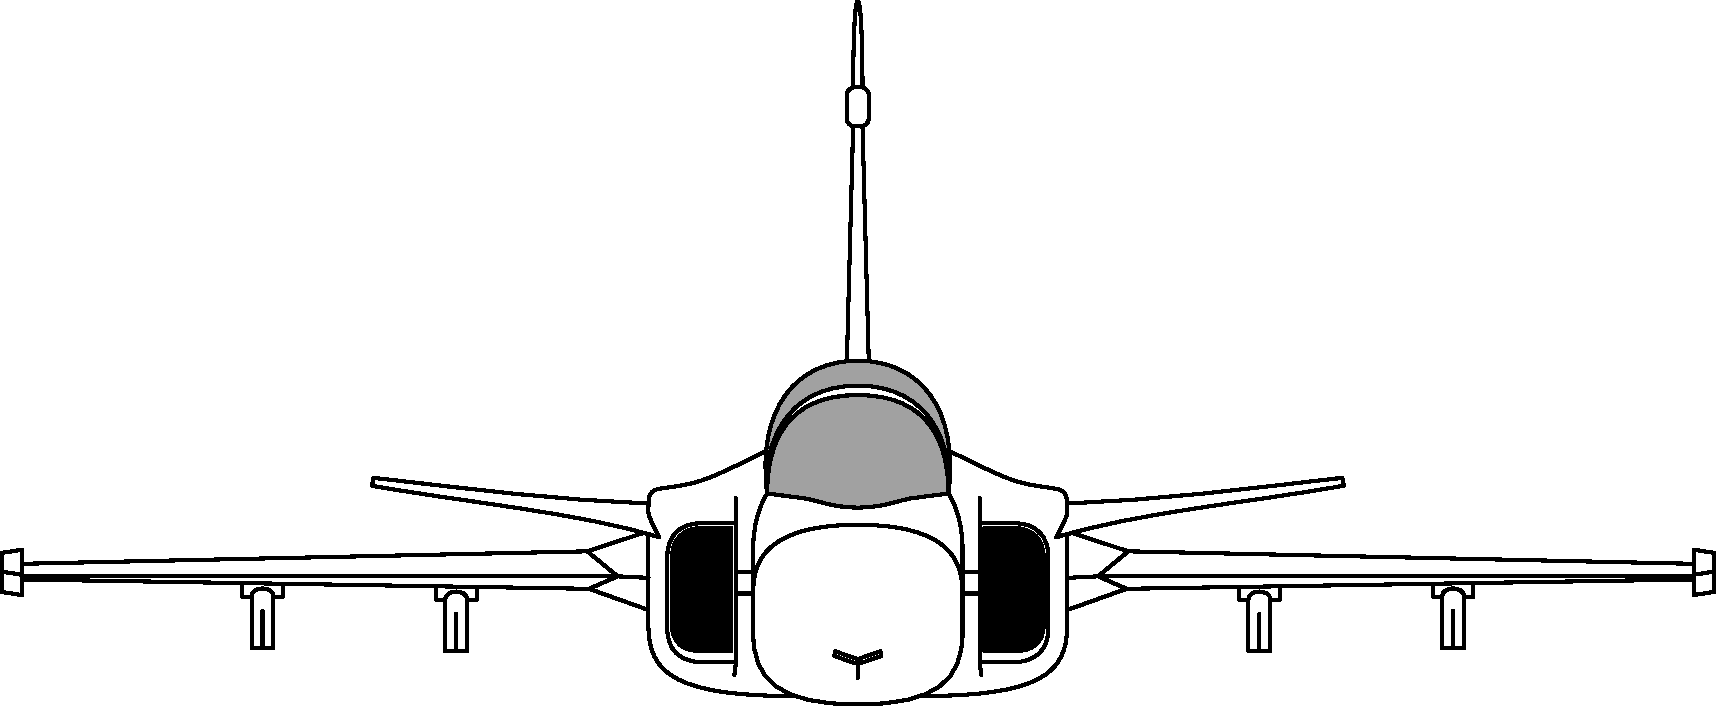
\includegraphics[width=0.7\textwidth]{figures/gripen}
%   \caption{An example figure. It is not normally advisable to include blocks around figures, and a block is only used here to give the figure size.}
%   \label{fig:example}
% \end{figure}

% \begin{figure}[htbp]
%   \centering
%   \subfigure[A vector image.
%   \label{fig:example_subfigure_1}]
%   {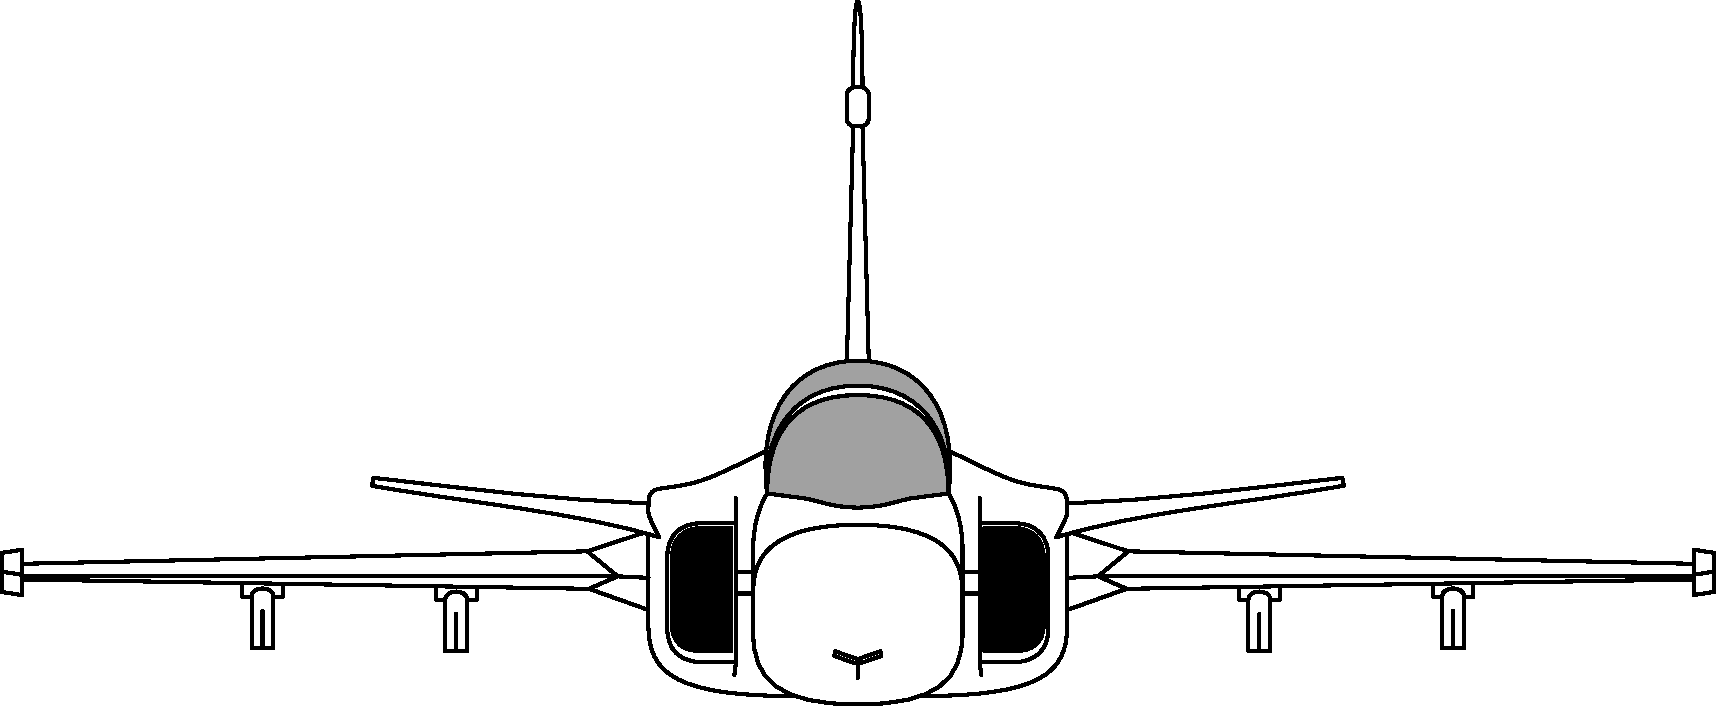
\includegraphics[width=0.48\textwidth]{figures/gripen.pdf}}
%   \hfill
%   \subfigure[A raster image.
%   \label{fig:example_subfigure_2}]
%   {
\includegraphics[width=0.48\textwidth]{figures/gripen.png}}
%   \caption{An example of how to use sub-figures.  The image was created by the author from a photograph of a Saab Gripen.}
%   \label{fig:example_subfigure}
% \end{figure}

% Note how much better the vector image in Figure~\ref{fig:example_subfigure_1} appears than
% the raster image in Figure~\ref{fig:example_subfigure_2}, especially when zoomed in or
% printed.  Additionally, the file with the vector image, \verb|figures/gripen.pdf| (3580
% bytes), is significantly smaller than the file with the raster image,
% \verb|figures/gripen.png| (11284 bytes), despite having higher quality.  The file
% \verb|figures/gripen.pdf| was generated using Inkscape with the original file being
% \verb|figures/gripen.svgz| (2935 bytes).

% \subsection{Abbreviations}
% \label{app:formatting_abbr}

% The \verb|acronym| package (included in the \verb|user_packages.tex| file) can be used to manage abbreviations used in the report. The first time an abbreviation appears in the report the description will be printed, after which only the abbreviation will appear. Three parameter options for this package are presented where it is included in the \verb|user_packages.tex| file. These options influence whether/how an abbreviations list is included in the \ac{PDF2} document when the \verb|abbreviations.tex| file is input into the \verb|report.tex| file.

% \begin{compactitem}
%     \item The \verb|[nolist]| setting does not print an abbreviation list in the \ac{PDF2}. Abbreviations are still used in-text in the same way as with the other options but no list is presented.
%     \item The \verb|[printonlyused]| setting is the current setting in this document. A list of abbreviations is included in the \ac{PDF2} where you input the \verb|abbreviations.tex| file. This list includes only the abbreviations that were used in the document.
%     \item When no parameter is included, i.e. the \verb|\usepackage{acronym}| command is used on its own, all the abbreviations defined in the \verb|abbreviations.tex| file are included in the list. This is usually not desired because it is beneficial to keep a general abbreviation dictionary that you can add to if additional abbreviations are required.
% \end{compactitem}

% The \href{https://ctan.math.washington.edu/tex-archive/macros/latex/contrib/acronym/acronym.pdf}{package documentation} contains detailed explanations regarding the available commands that can be used. A few useful commands include: 
% \begin{compactitem}
%     \item \verb|\ac| -- The most commonly used command; it will print the description of the abbreviation the first time you use it, after which it will print only the abbreviation. The first word will start with a lowercase letter unless it was defined to start with an uppercase letter in the \verb|\acro| command in the \verb|abbreviations.tex| file. For example, \ac{SNR} and \ac{SNR}.
%     \item \verb|\Ac| -- It functions the same as the \verb|\ac| command but will print the first word starting with an uppercase letter; this is typically used when a sentence starts with an abbreviation. For example, \Ac{2D} and \Ac{2D}. \textit{All following commands use the same lowercase/uppercase principle.}
%     \item \verb|\acf| -- Prints the description even if the abbreviation was used earlier in the document. For example, \acf{PDF2} and \Acf{PDF2}.
%     \item \verb|\acp| -- Prints the plural of an abbreviation. For example, \acp{LED} instead of the singular \acf{LED}. 
%     \item \verb|\acs| -- Prints only the abbreviation even if it has not been previously used. This is useful when an abbreviation is included in a figure/table caption and a list of figures/tables is included. In such a scenario, the description would usually only be printed in the list of figures/tables. When using the \verb|\acs| command instead of just the \verb|\ac| command, the description will be printed the first time the abbreviation appears in the text rather than in the list of figures/tables.
% \end{compactitem}

% \subsection{Bibtex}
% \label{app:bibtex}

% The \href{https://ieeeauthorcenter.ieee.org/wp-content/uploads/IEEE-Reference-Guide.pdf}{\Ac{IEEE} reference style} shoud be used when citing sources and for the reference list. Sources are numbered according to the order in which they appear in the document and are cited by placing the number in square brackets, eg. \cite{duPlessis_pracx_data}.

% Managing your sources can be done by defining all sources in the \verb|references.bib| BibTeX file and using the \verb|\cite{}| command to cite a source. The \href{https://www.bibtex.com/g/bibtex-format/}{Bibtex format guide} provides an explanation for the BibTeX format. 

% %% Acronyms without printing list
% % \usepackage[nolist]{acronym}
% %% Acronyms printing only the ones used in the document
% % \usepackage[printonlyused]{acronym}
% %% Acronyms printing everything in list
% % \usepackage{acronym}

% \section{Data}
% \label{app:data}

% Avoid adding excessive amounts of additional data, unless the instructions specifically ask for it.


\end{document}
 